
\begin{frame}[fragile]
\frametitle{Demo 05: Agregar un RadioGroup}
\begin{columns}
\column{0.80\linewidth}
Del Repositorio Github:
\begin{itemize}
\item Copiar el archivo MainActivity\_Demo05.java (dentro del Folder códigosJAVA) al mismo directorio donde esta el MainActivity.java
\item Copiar el archivo activity\_main\_demo05.xml (dentro del Folder Carpeta\_layout) al mismo directorio donde esta el activity\_main.xml
\item Copiar los archivos \textit{cgup.jpg} y \textit{logo\_upv\_2019.png} localizados dentro de la folder \textit{Carpeta\_drawable} en el directorio \textit{res/drawable} del proyecto de AS.
\item Modificar en el archivo AndroidManifest.xml la cadena \textit{.MainActivity\_Demo04} por \textit{.MainActivity\_Demo05}
\end{itemize}

\begin{block}{Demo \#05}
Muestra una App con un RadioGroup. El ImageView cambia basado en la seleccion del usuario.    
\end{block}


\column{0.20\linewidth}

\begin{center}
 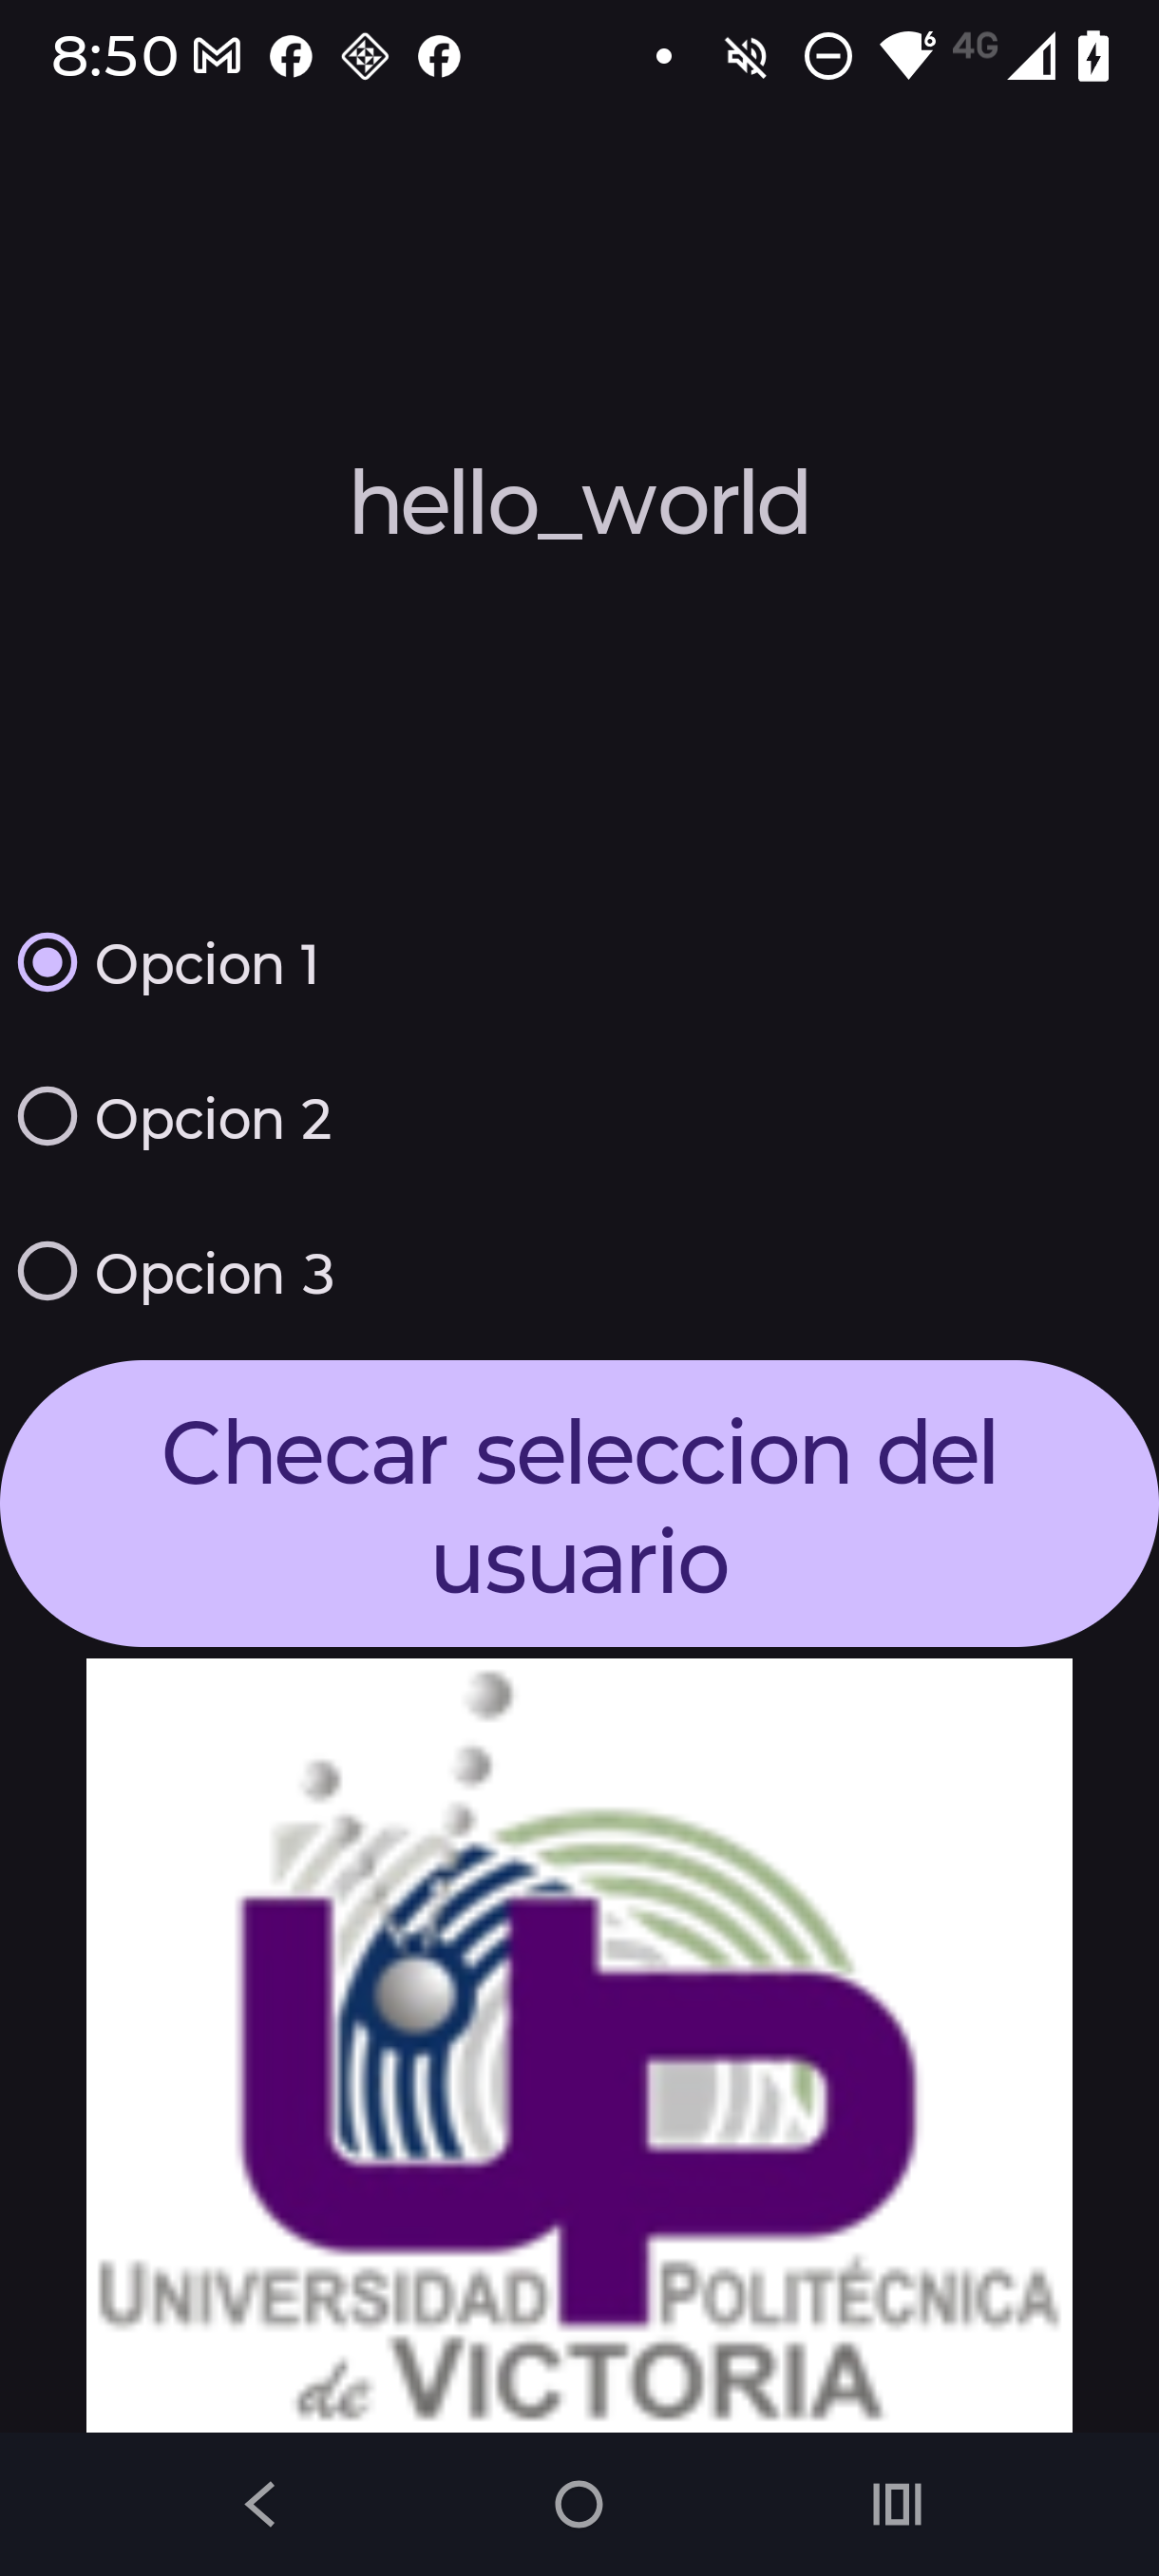
\includegraphics[width=0.98\textwidth]{02_TallerCBTis/figs/Demo05}
\end{center}

\end{columns}

\end{frame}


